\documentclass[1p]{elsarticle_modified}
%\bibliographystyle{elsarticle-num}

%\usepackage[colorlinks]{hyperref}
%\usepackage{abbrmath_seonhwa} %\Abb, \Ascr, \Acal ,\Abf, \Afrak
\usepackage{amsfonts}
\usepackage{amssymb}
\usepackage{amsmath}
\usepackage{amsthm}
\usepackage{scalefnt}
\usepackage{amsbsy}
\usepackage{kotex}
\usepackage{caption}
\usepackage{subfig}
\usepackage{color}
\usepackage{graphicx}
\usepackage{xcolor} %% white, black, red, green, blue, cyan, magenta, yellow
\usepackage{float}
\usepackage{setspace}
\usepackage{hyperref}

\usepackage{tikz}
\usetikzlibrary{arrows}

\usepackage{multirow}
\usepackage{array} % fixed length table
\usepackage{hhline}

%%%%%%%%%%%%%%%%%%%%%
\makeatletter
\renewcommand*\env@matrix[1][\arraystretch]{%
	\edef\arraystretch{#1}%
	\hskip -\arraycolsep
	\let\@ifnextchar\new@ifnextchar
	\array{*\c@MaxMatrixCols c}}
\makeatother %https://tex.stackexchange.com/questions/14071/how-can-i-increase-the-line-spacing-in-a-matrix
%%%%%%%%%%%%%%%

\usepackage[normalem]{ulem}

\newcommand{\msout}[1]{\ifmmode\text{\sout{\ensuremath{#1}}}\else\sout{#1}\fi}
%SOURCE: \msout is \stkout macro in https://tex.stackexchange.com/questions/20609/strikeout-in-math-mode

\newcommand{\cancel}[1]{
	\ifmmode
	{\color{red}\msout{#1}}
	\else
	{\color{red}\sout{#1}}
	\fi
}

\newcommand{\add}[1]{
	{\color{blue}\uwave{#1}}
}

\newcommand{\replace}[2]{
	\ifmmode
	{\color{red}\msout{#1}}{\color{blue}\uwave{#2}}
	\else
	{\color{red}\sout{#1}}{\color{blue}\uwave{#2}}
	\fi
}

\newcommand{\Sol}{\mathcal{S}} %segment
\newcommand{\D}{D} %diagram
\newcommand{\A}{\mathcal{A}} %arc


%%%%%%%%%%%%%%%%%%%%%%%%%%%%%5 test

\def\sl{\operatorname{\textup{SL}}(2,\Cbb)}
\def\psl{\operatorname{\textup{PSL}}(2,\Cbb)}
\def\quan{\mkern 1mu \triangleright \mkern 1mu}

\theoremstyle{definition}
\newtheorem{thm}{Theorem}[section]
\newtheorem{prop}[thm]{Proposition}
\newtheorem{lem}[thm]{Lemma}
\newtheorem{ques}[thm]{Question}
\newtheorem{cor}[thm]{Corollary}
\newtheorem{defn}[thm]{Definition}
\newtheorem{exam}[thm]{Example}
\newtheorem{rmk}[thm]{Remark}
\newtheorem{alg}[thm]{Algorithm}

\newcommand{\I}{\sqrt{-1}}
\begin{document}

%\begin{frontmatter}
%
%\title{Boundary parabolic representations of knots up to 8 crossings}
%
%%% Group authors per affiliation:
%\author{Yunhi Cho} 
%\address{Department of Mathematics, University of Seoul, Seoul, Korea}
%\ead{yhcho@uos.ac.kr}
%
%
%\author{Seonhwa Kim} %\fnref{s_kim}}
%\address{Center for Geometry and Physics, Institute for Basic Science, Pohang, 37673, Korea}
%\ead{ryeona17@ibs.re.kr}
%
%\author{Hyuk Kim}
%\address{Department of Mathematical Sciences, Seoul National University, Seoul 08826, Korea}
%\ead{hyukkim@snu.ac.kr}
%
%\author{Seokbeom Yoon}
%\address{Department of Mathematical Sciences, Seoul National University, Seoul, 08826,  Korea}
%\ead{sbyoon15@snu.ac.kr}
%
%\begin{abstract}
%We find all boundary parabolic representation of knots up to 8 crossings.
%
%\end{abstract}
%\begin{keyword}
%    \MSC[2010] 57M25 
%\end{keyword}
%
%\end{frontmatter}

%\linenumbers
%\tableofcontents
%
\newcommand\colored[1]{\textcolor{white}{\rule[-0.35ex]{0.8em}{1.4ex}}\kern-0.8em\color{red} #1}%
%\newcommand\colored[1]{\textcolor{white}{ #1}\kern-2.17ex	\textcolor{white}{ #1}\kern-1.81ex	\textcolor{white}{ #1}\kern-2.15ex\color{red}#1	}

{\Large $\underline{12a_{0862}~(K12a_{0862})}$}

\setlength{\tabcolsep}{10pt}
\renewcommand{\arraystretch}{1.6}
\vspace{1cm}\begin{tabular}{m{100pt}>{\centering\arraybackslash}m{274pt}}
\multirow{5}{120pt}{
	\centering
	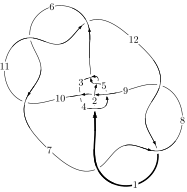
\includegraphics[width=112pt]{../../../GIT/diagram.site/Diagrams/png/1663_12a_0862.png}\\
\ \ \ A knot diagram\footnotemark}&
\allowdisplaybreaks
\textbf{Linearized knot diagam} \\
\cline{2-2}
 &
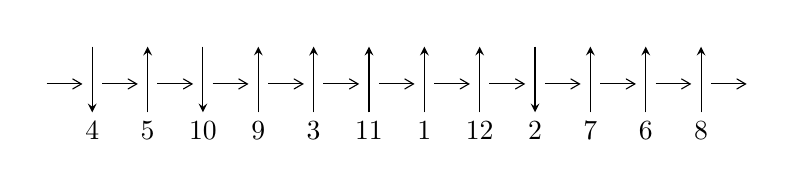
\begin{tikzpicture}[x=20pt, y=17pt]
	% nodes
	\node (C0) at (0, 0) {};
	\node (C1) at (1, 0) {};
	\node (C1U) at (1, +1) {};
	\node (C1D) at (1, -1) {4};

	\node (C2) at (2, 0) {};
	\node (C2U) at (2, +1) {};
	\node (C2D) at (2, -1) {5};

	\node (C3) at (3, 0) {};
	\node (C3U) at (3, +1) {};
	\node (C3D) at (3, -1) {10};

	\node (C4) at (4, 0) {};
	\node (C4U) at (4, +1) {};
	\node (C4D) at (4, -1) {9};

	\node (C5) at (5, 0) {};
	\node (C5U) at (5, +1) {};
	\node (C5D) at (5, -1) {3};

	\node (C6) at (6, 0) {};
	\node (C6U) at (6, +1) {};
	\node (C6D) at (6, -1) {11};

	\node (C7) at (7, 0) {};
	\node (C7U) at (7, +1) {};
	\node (C7D) at (7, -1) {1};

	\node (C8) at (8, 0) {};
	\node (C8U) at (8, +1) {};
	\node (C8D) at (8, -1) {12};

	\node (C9) at (9, 0) {};
	\node (C9U) at (9, +1) {};
	\node (C9D) at (9, -1) {2};

	\node (C10) at (10, 0) {};
	\node (C10U) at (10, +1) {};
	\node (C10D) at (10, -1) {7};

	\node (C11) at (11, 0) {};
	\node (C11U) at (11, +1) {};
	\node (C11D) at (11, -1) {6};

	\node (C12) at (12, 0) {};
	\node (C12U) at (12, +1) {};
	\node (C12D) at (12, -1) {8};
	\node (C13) at (13, 0) {};

	% arrows
	\draw[->,>={angle 60}]
	(C0) edge (C1) (C1) edge (C2) (C2) edge (C3) (C3) edge (C4) (C4) edge (C5) (C5) edge (C6) (C6) edge (C7) (C7) edge (C8) (C8) edge (C9) (C9) edge (C10) (C10) edge (C11) (C11) edge (C12) (C12) edge (C13) ;	\draw[->,>=stealth]
	(C1U) edge (C1D) (C2D) edge (C2U) (C3U) edge (C3D) (C4D) edge (C4U) (C5D) edge (C5U) (C6D) edge (C6U) (C7D) edge (C7U) (C8D) edge (C8U) (C9U) edge (C9D) (C10D) edge (C10U) (C11D) edge (C11U) (C12D) edge (C12U) ;
	\end{tikzpicture} \\
\hhline{~~} \\& 
\textbf{Solving Sequence} \\ \cline{2-2} 
 &
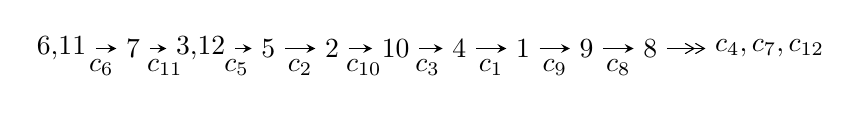
\begin{tikzpicture}[x=23pt, y=7pt]
	% node
	\node (A0) at (-1/8, 0) {6,11};
	\node (A1) at (1, 0) {7};
	\node (A2) at (33/16, 0) {3,12};
	\node (A3) at (25/8, 0) {5};
	\node (A4) at (33/8, 0) {2};
	\node (A5) at (41/8, 0) {10};
	\node (A6) at (49/8, 0) {4};
	\node (A7) at (57/8, 0) {1};
	\node (A8) at (65/8, 0) {9};
	\node (A9) at (73/8, 0) {8};
	\node (C1) at (1/2, -1) {$c_{6}$};
	\node (C2) at (3/2, -1) {$c_{11}$};
	\node (C3) at (21/8, -1) {$c_{5}$};
	\node (C4) at (29/8, -1) {$c_{2}$};
	\node (C5) at (37/8, -1) {$c_{10}$};
	\node (C6) at (45/8, -1) {$c_{3}$};
	\node (C7) at (53/8, -1) {$c_{1}$};
	\node (C8) at (61/8, -1) {$c_{9}$};
	\node (C9) at (69/8, -1) {$c_{8}$};
	\node (A10) at (11, 0) {$c_{4},c_{7},c_{12}$};

	% edge
	\draw[->,>=stealth]	
	(A0) edge (A1) (A1) edge (A2) (A2) edge (A3) (A3) edge (A4) (A4) edge (A5) (A5) edge (A6) (A6) edge (A7) (A7) edge (A8) (A8) edge (A9) ;
	\draw[->>,>={angle 60}]	
	(A9) edge (A10);
\end{tikzpicture} \\ 

\end{tabular} \\

\footnotetext{
The image of knot diagram is generated by the software ``\textbf{Draw programme}" developed by Andrew Bartholomew(\url{http://www.layer8.co.uk/maths/draw/index.htm\#Running-draw}), where we modified some parts for our purpose(\url{https://github.com/CATsTAILs/LinksPainter}).
}\phantom \\ \newline 
\centering \textbf{Ideals for irreducible components\footnotemark of $X_{\text{par}}$} 
 
\begin{align*}
I^u_{1}&=\langle 
-2.41366\times10^{15} u^{41}-3.88647\times10^{15} u^{40}+\cdots+2.70070\times10^{16} b-2.38778\times10^{16},\\
\phantom{I^u_{1}}&\phantom{= \langle  }3.90532\times10^{16} u^{41}+4.65482\times10^{15} u^{40}+\cdots+1.08028\times10^{17} a-2.34376\times10^{17},\;u^{42}+u^{41}+\cdots+5 u+1\rangle \\
I^u_{2}&=\langle 
5.71537\times10^{60} u^{59}+9.40318\times10^{60} u^{58}+\cdots+1.05278\times10^{62} b-1.05491\times10^{62},\\
\phantom{I^u_{2}}&\phantom{= \langle  }5.50355\times10^{62} u^{59}+1.37835\times10^{63} u^{58}+\cdots+1.78973\times10^{63} a+1.81400\times10^{64},\;u^{60}+u^{59}+\cdots+96 u+17\rangle \\
I^u_{3}&=\langle 
-9 a^4 u+137 a^4-670 a^3 u-515 a^3+896 a^2 u-428 a^2+1221 a u+725 b-703 a-211 u+1198,\\
\phantom{I^u_{3}}&\phantom{= \langle  }a^5-5 a^4 u-4 a^4+9 a^3 u-2 a^3+6 a^2 u-6 a u+7 a-1,\;u^2+1\rangle \\
I^u_{4}&=\langle 
b-1,\;4 a+3,\;u+1\rangle \\
\\
\end{align*}
\raggedright * 4 irreducible components of $\dim_{\mathbb{C}}=0$, with total 113 representations.\\
\footnotetext{All coefficients of polynomials are rational numbers. But the coefficients are sometimes approximated in decimal forms when there is not enough margin.}
\newpage
\renewcommand{\arraystretch}{1}
\centering \section*{I. $I^u_{1}= \langle -2.41\times10^{15} u^{41}-3.89\times10^{15} u^{40}+\cdots+2.70\times10^{16} b-2.39\times10^{16},\;3.91\times10^{16} u^{41}+4.65\times10^{15} u^{40}+\cdots+1.08\times10^{17} a-2.34\times10^{17},\;u^{42}+u^{41}+\cdots+5 u+1 \rangle$}
\flushleft \textbf{(i) Arc colorings}\\
\begin{tabular}{m{7pt} m{180pt} m{7pt} m{180pt} }
\flushright $a_{6}=$&$\begin{pmatrix}1\\0\end{pmatrix}$ \\
\flushright $a_{11}=$&$\begin{pmatrix}0\\u\end{pmatrix}$ \\
\flushright $a_{7}=$&$\begin{pmatrix}1\\- u^2\end{pmatrix}$ \\
\flushright $a_{3}=$&$\begin{pmatrix}-0.361511 u^{41}-0.0430891 u^{40}+\cdots-6.03379 u+2.16959\\0.0893718 u^{41}+0.143906 u^{40}+\cdots-0.178892 u+0.884133\end{pmatrix}$ \\
\flushright $a_{12}=$&$\begin{pmatrix}u\\u\end{pmatrix}$ \\
\flushright $a_{5}=$&$\begin{pmatrix}-0.315904 u^{41}+0.0662626 u^{40}+\cdots-5.94901 u+3.22945\\0.174739 u^{41}+0.111875 u^{40}+\cdots+0.0944736 u+0.995695\end{pmatrix}$ \\
\flushright $a_{2}=$&$\begin{pmatrix}-0.0742984 u^{41}-0.106140 u^{40}+\cdots+2.43989 u-0.719779\\-0.188640 u^{41}+0.154687 u^{40}+\cdots+1.14048 u+0.0824999\end{pmatrix}$ \\
\flushright $a_{10}=$&$\begin{pmatrix}- u\\u^3+u\end{pmatrix}$ \\
\flushright $a_{4}=$&$\begin{pmatrix}-0.155243 u^{41}+0.143329 u^{40}+\cdots-4.42970 u+2.56854\\-0.0568312 u^{41}+0.0634325 u^{40}+\cdots-1.67596 u+0.465338\end{pmatrix}$ \\
\flushright $a_{1}=$&$\begin{pmatrix}-0.0312500 u^{41}-0.0312500 u^{40}+\cdots-0.156250 u^{2}-2.03125 u\\-0.0312500 u^{41}-0.0312500 u^{40}+\cdots-0.156250 u^{2}-1.03125 u\end{pmatrix}$ \\
\flushright $a_{9}=$&$\begin{pmatrix}0.0312500 u^{40}+0.0312500 u^{39}+\cdots+0.156250 u+1.03125\\0.0312500 u^{40}+0.0312500 u^{39}+\cdots+0.156250 u+0.0312500\end{pmatrix}$ \\
\flushright $a_{8}=$&$\begin{pmatrix}0.0312500 u^{40}+0.0312500 u^{39}+\cdots+0.156250 u+1.03125\\0.0312500 u^{40}+0.0312500 u^{39}+\cdots+0.156250 u+0.0312500\end{pmatrix}$\\&\end{tabular}
\flushleft \textbf{(ii) Obstruction class $= -1$}\\~\\
\flushleft \textbf{(iii) Cusp Shapes $= -\frac{789866485036270413}{432111644840574976} u^{41}-\frac{3177961663845613}{3375872225316992} u^{40}+\cdots-\frac{515566611610676781}{108027911210143744} u+\frac{1182572220834268723}{432111644840574976}$}\\~\\
\newpage\renewcommand{\arraystretch}{1}
\flushleft \textbf{(iv) u-Polynomials at the component}\newline \\
\begin{tabular}{m{50pt}|m{274pt}}
Crossings & \hspace{64pt}u-Polynomials at each crossing \\
\hline $$\begin{aligned}c_{1}\end{aligned}$$&$\begin{aligned}
&u^{42}-7 u^{41}+\cdots+44 u+32
\end{aligned}$\\
\hline $$\begin{aligned}c_{2},c_{5}\end{aligned}$$&$\begin{aligned}
&u^{42}+2 u^{41}+\cdots+175 u-16
\end{aligned}$\\
\hline $$\begin{aligned}c_{3}\end{aligned}$$&$\begin{aligned}
&2(2 u^{42}+7 u^{41}+\cdots+62575 u-9794)
\end{aligned}$\\
\hline $$\begin{aligned}c_{4}\end{aligned}$$&$\begin{aligned}
&2(2 u^{42}+19 u^{41}+\cdots+6823 u+542)
\end{aligned}$\\
\hline $$\begin{aligned}c_{6},c_{7},c_{8}\\c_{10},c_{11},c_{12}\end{aligned}$$&$\begin{aligned}
&u^{42}- u^{41}+\cdots-5 u+1
\end{aligned}$\\
\hline $$\begin{aligned}c_{9}\end{aligned}$$&$\begin{aligned}
&u^{42}-11 u^{41}+\cdots+12 u-4
\end{aligned}$\\
\hline
\end{tabular}\\~\\
\newpage\renewcommand{\arraystretch}{1}
\flushleft \textbf{(v) Riley Polynomials at the component}\newline \\
\begin{tabular}{m{50pt}|m{274pt}}
Crossings & \hspace{64pt}Riley Polynomials at each crossing \\
\hline $$\begin{aligned}c_{1}\end{aligned}$$&$\begin{aligned}
&y^{42}+3 y^{41}+\cdots-8784 y+1024
\end{aligned}$\\
\hline $$\begin{aligned}c_{2},c_{5}\end{aligned}$$&$\begin{aligned}
&y^{42}-30 y^{41}+\cdots-15201 y+256
\end{aligned}$\\
\hline $$\begin{aligned}c_{3}\end{aligned}$$&$\begin{aligned}
&4(4 y^{42}-101 y^{41}+\cdots+6.32683\times10^{8} y+9.59224\times10^{7})
\end{aligned}$\\
\hline $$\begin{aligned}c_{4}\end{aligned}$$&$\begin{aligned}
&4(4 y^{42}-181 y^{41}+\cdots-8215501 y+293764)
\end{aligned}$\\
\hline $$\begin{aligned}c_{6},c_{7},c_{8}\\c_{10},c_{11},c_{12}\end{aligned}$$&$\begin{aligned}
&y^{42}+45 y^{41}+\cdots+11 y+1
\end{aligned}$\\
\hline $$\begin{aligned}c_{9}\end{aligned}$$&$\begin{aligned}
&y^{42}+3 y^{41}+\cdots+40 y+16
\end{aligned}$\\
\hline
\end{tabular}\\~\\
\newpage\flushleft \textbf{(vi) Complex Volumes and Cusp Shapes}
$$\begin{array}{c|c|c}  
\text{Solutions to }I^u_{1}& \I (\text{vol} + \sqrt{-1}CS) & \text{Cusp shape}\\
 \hline 
\begin{aligned}
u &= -0.848250 + 0.512070 I \\
a &= \phantom{-}0.207456 + 0.529240 I \\
b &= -1.095070 - 0.103799 I\end{aligned}
 & \phantom{-}3.98284 - 0.00703 I & \phantom{-}16.2188 - 8.0603 I \\ \hline\begin{aligned}
u &= -0.848250 - 0.512070 I \\
a &= \phantom{-}0.207456 - 0.529240 I \\
b &= -1.095070 + 0.103799 I\end{aligned}
 & \phantom{-}3.98284 + 0.00703 I & \phantom{-}16.2188 + 8.0603 I \\ \hline\begin{aligned}
u &= \phantom{-}0.800314 + 0.304736 I \\
a &= \phantom{-}0.829077 - 1.057030 I \\
b &= -1.330470 - 0.471690 I\end{aligned}
 & \phantom{-}5.06478 + 9.22584 I & \phantom{-}10.05550 - 8.03379 I \\ \hline\begin{aligned}
u &= \phantom{-}0.800314 - 0.304736 I \\
a &= \phantom{-}0.829077 + 1.057030 I \\
b &= -1.330470 + 0.471690 I\end{aligned}
 & \phantom{-}5.06478 - 9.22584 I & \phantom{-}10.05550 + 8.03379 I \\ \hline\begin{aligned}
u &= -1.14704\phantom{ +0.000000I} \\
a &= \phantom{-}0.588362\phantom{ +0.000000I} \\
b &= -0.957842\phantom{ +0.000000I}\end{aligned}
 & \phantom{-}3.16700\phantom{ +0.000000I} & -41.0100\phantom{ +0.000000I} \\ \hline\begin{aligned}
u &= -0.012618 + 1.267560 I \\
a &= -0.257462 - 0.166119 I \\
b &= -1.55639 - 0.20562 I\end{aligned}
 & \phantom{-}1.02826 + 4.26198 I & \phantom{-0.000000 } 0 \\ \hline\begin{aligned}
u &= -0.012618 - 1.267560 I \\
a &= -0.257462 + 0.166119 I \\
b &= -1.55639 + 0.20562 I\end{aligned}
 & \phantom{-}1.02826 - 4.26198 I & \phantom{-0.000000 } 0 \\ \hline\begin{aligned}
u &= -0.034204 + 0.691000 I \\
a &= -0.842871 + 0.389564 I \\
b &= -1.348420 + 0.231077 I\end{aligned}
 & \phantom{-}3.66010 - 4.50065 I & \phantom{-}13.13111 + 5.04481 I \\ \hline\begin{aligned}
u &= -0.034204 - 0.691000 I \\
a &= -0.842871 - 0.389564 I \\
b &= -1.348420 - 0.231077 I\end{aligned}
 & \phantom{-}3.66010 + 4.50065 I & \phantom{-}13.13111 - 5.04481 I \\ \hline\begin{aligned}
u &= \phantom{-}0.616502 + 0.228755 I \\
a &= -0.376552 + 0.322880 I \\
b &= \phantom{-}0.092715 + 0.998112 I\end{aligned}
 & \phantom{-}0.67504 + 4.06826 I & \phantom{-}8.30605 - 8.37246 I\\
 \hline 
 \end{array}$$\newpage$$\begin{array}{c|c|c}  
\text{Solutions to }I^u_{1}& \I (\text{vol} + \sqrt{-1}CS) & \text{Cusp shape}\\
 \hline 
\begin{aligned}
u &= \phantom{-}0.616502 - 0.228755 I \\
a &= -0.376552 - 0.322880 I \\
b &= \phantom{-}0.092715 - 0.998112 I\end{aligned}
 & \phantom{-}0.67504 - 4.06826 I & \phantom{-}8.30605 + 8.37246 I \\ \hline\begin{aligned}
u &= \phantom{-}0.631212 + 0.066643 I \\
a &= -1.208440 + 0.639819 I \\
b &= \phantom{-}1.39513 + 0.51274 I\end{aligned}
 & \phantom{-}4.64462 + 1.79449 I & \phantom{-}16.6728 - 4.4347 I \\ \hline\begin{aligned}
u &= \phantom{-}0.631212 - 0.066643 I \\
a &= -1.208440 - 0.639819 I \\
b &= \phantom{-}1.39513 - 0.51274 I\end{aligned}
 & \phantom{-}4.64462 - 1.79449 I & \phantom{-}16.6728 + 4.4347 I \\ \hline\begin{aligned}
u &= -0.22206 + 1.39802 I \\
a &= \phantom{-}0.703692 - 0.255357 I \\
b &= \phantom{-}1.80328 + 0.31389 I\end{aligned}
 & -4.00787 - 4.08479 I & \phantom{-0.000000 } 0 \\ \hline\begin{aligned}
u &= -0.22206 - 1.39802 I \\
a &= \phantom{-}0.703692 + 0.255357 I \\
b &= \phantom{-}1.80328 - 0.31389 I\end{aligned}
 & -4.00787 + 4.08479 I & \phantom{-0.000000 } 0 \\ \hline\begin{aligned}
u &= -0.14844 + 1.41232 I \\
a &= \phantom{-}0.821579 + 1.118480 I \\
b &= \phantom{-}0.75327 + 1.20186 I\end{aligned}
 & -6.98470 - 0.19701 I & \phantom{-0.000000 } 0 \\ \hline\begin{aligned}
u &= -0.14844 - 1.41232 I \\
a &= \phantom{-}0.821579 - 1.118480 I \\
b &= \phantom{-}0.75327 - 1.20186 I\end{aligned}
 & -6.98470 + 0.19701 I & \phantom{-0.000000 } 0 \\ \hline\begin{aligned}
u &= -0.27736 + 1.41903 I \\
a &= \phantom{-}0.20943 - 1.78788 I \\
b &= \phantom{-}1.42598 - 0.91461 I\end{aligned}
 & -5.04656 - 8.51889 I & \phantom{-0.000000 } 0 \\ \hline\begin{aligned}
u &= -0.27736 - 1.41903 I \\
a &= \phantom{-}0.20943 + 1.78788 I \\
b &= \phantom{-}1.42598 + 0.91461 I\end{aligned}
 & -5.04656 + 8.51889 I & \phantom{-0.000000 } 0 \\ \hline\begin{aligned}
u &= \phantom{-}0.18419 + 1.44787 I \\
a &= \phantom{-}0.67100 - 1.30177 I \\
b &= \phantom{-}0.747156 - 0.401730 I\end{aligned}
 & -8.12596 + 3.90378 I & \phantom{-0.000000 } 0\\
 \hline 
 \end{array}$$\newpage$$\begin{array}{c|c|c}  
\text{Solutions to }I^u_{1}& \I (\text{vol} + \sqrt{-1}CS) & \text{Cusp shape}\\
 \hline 
\begin{aligned}
u &= \phantom{-}0.18419 - 1.44787 I \\
a &= \phantom{-}0.67100 + 1.30177 I \\
b &= \phantom{-}0.747156 + 0.401730 I\end{aligned}
 & -8.12596 - 3.90378 I & \phantom{-0.000000 } 0 \\ \hline\begin{aligned}
u &= \phantom{-}0.24426 + 1.44190 I \\
a &= -0.87161 + 1.77499 I \\
b &= \phantom{-}1.133290 + 0.182062 I\end{aligned}
 & -7.23578 + 5.67907 I & \phantom{-0.000000 } 0 \\ \hline\begin{aligned}
u &= \phantom{-}0.24426 - 1.44190 I \\
a &= -0.87161 - 1.77499 I \\
b &= \phantom{-}1.133290 - 0.182062 I\end{aligned}
 & -7.23578 - 5.67907 I & \phantom{-0.000000 } 0 \\ \hline\begin{aligned}
u &= -0.513585\phantom{ +0.000000I} \\
a &= -6.41966\phantom{ +0.000000I} \\
b &= \phantom{-}1.04008\phantom{ +0.000000I}\end{aligned}
 & \phantom{-}2.62940\phantom{ +0.000000I} & -41.1690\phantom{ +0.000000I} \\ \hline\begin{aligned}
u &= -0.491329 + 0.139176 I \\
a &= \phantom{-}0.845547 - 0.468260 I \\
b &= \phantom{-}0.133518 - 0.061566 I\end{aligned}
 & \phantom{-}1.019720 - 0.352110 I & \phantom{-}10.07407 + 1.64611 I \\ \hline\begin{aligned}
u &= -0.491329 - 0.139176 I \\
a &= \phantom{-}0.845547 + 0.468260 I \\
b &= \phantom{-}0.133518 + 0.061566 I\end{aligned}
 & \phantom{-}1.019720 + 0.352110 I & \phantom{-}10.07407 - 1.64611 I \\ \hline\begin{aligned}
u &= \phantom{-}0.41236 + 1.44280 I \\
a &= \phantom{-}0.077835 - 1.227670 I \\
b &= -1.175080 - 0.389371 I\end{aligned}
 & -7.08053 + 10.21340 I & \phantom{-0.000000 } 0 \\ \hline\begin{aligned}
u &= \phantom{-}0.41236 - 1.44280 I \\
a &= \phantom{-}0.077835 + 1.227670 I \\
b &= -1.175080 + 0.389371 I\end{aligned}
 & -7.08053 - 10.21340 I & \phantom{-0.000000 } 0 \\ \hline\begin{aligned}
u &= -0.32208 + 1.46578 I \\
a &= -0.67927 - 1.33639 I \\
b &= -0.074878 - 1.346880 I\end{aligned}
 & -10.3464 - 11.3808 I & \phantom{-0.000000 } 0 \\ \hline\begin{aligned}
u &= -0.32208 - 1.46578 I \\
a &= -0.67927 + 1.33639 I \\
b &= -0.074878 + 1.346880 I\end{aligned}
 & -10.3464 + 11.3808 I & \phantom{-0.000000 } 0\\
 \hline 
 \end{array}$$\newpage$$\begin{array}{c|c|c}  
\text{Solutions to }I^u_{1}& \I (\text{vol} + \sqrt{-1}CS) & \text{Cusp shape}\\
 \hline 
\begin{aligned}
u &= -0.39351 + 1.46640 I \\
a &= -0.02848 + 1.76784 I \\
b &= -1.40317 + 0.63323 I\end{aligned}
 & -6.1337 - 18.1779 I & \phantom{-0.000000 } 0 \\ \hline\begin{aligned}
u &= -0.39351 - 1.46640 I \\
a &= -0.02848 - 1.76784 I \\
b &= -1.40317 - 0.63323 I\end{aligned}
 & -6.1337 + 18.1779 I & \phantom{-0.000000 } 0 \\ \hline\begin{aligned}
u &= \phantom{-}0.28895 + 1.49339 I \\
a &= -0.022490 + 0.757026 I \\
b &= -0.100578 + 0.571615 I\end{aligned}
 & -10.21670 + 6.45809 I & \phantom{-0.000000 } 0 \\ \hline\begin{aligned}
u &= \phantom{-}0.28895 - 1.49339 I \\
a &= -0.022490 - 0.757026 I \\
b &= -0.100578 - 0.571615 I\end{aligned}
 & -10.21670 - 6.45809 I & \phantom{-0.000000 } 0 \\ \hline\begin{aligned}
u &= -0.05826 + 1.54611 I \\
a &= -0.015563 + 1.355460 I \\
b &= -0.615041 + 0.997986 I\end{aligned}
 & -14.1579 + 0.2551 I & \phantom{-0.000000 } 0 \\ \hline\begin{aligned}
u &= -0.05826 - 1.54611 I \\
a &= -0.015563 - 1.355460 I \\
b &= -0.615041 - 0.997986 I\end{aligned}
 & -14.1579 - 0.2551 I & \phantom{-0.000000 } 0 \\ \hline\begin{aligned}
u &= \phantom{-}0.040969 + 0.400596 I \\
a &= \phantom{-}1.18528 - 1.17600 I \\
b &= \phantom{-}0.058208 - 0.592373 I\end{aligned}
 & -0.83418 - 1.45922 I & \phantom{-}1.76553 + 2.89021 I \\ \hline\begin{aligned}
u &= \phantom{-}0.040969 - 0.400596 I \\
a &= \phantom{-}1.18528 + 1.17600 I \\
b &= \phantom{-}0.058208 + 0.592373 I\end{aligned}
 & -0.83418 + 1.45922 I & \phantom{-}1.76553 - 2.89021 I \\ \hline\begin{aligned}
u &= \phantom{-}0.07832 + 1.61476 I \\
a &= -0.500043 - 0.967191 I \\
b &= -0.946634 - 0.650726 I\end{aligned}
 & -13.0094 + 6.1124 I & \phantom{-0.000000 } 0 \\ \hline\begin{aligned}
u &= \phantom{-}0.07832 - 1.61476 I \\
a &= -0.500043 + 0.967191 I \\
b &= -0.946634 + 0.650726 I\end{aligned}
 & -13.0094 - 6.1124 I & \phantom{-0.000000 } 0\\
 \hline 
 \end{array}$$\newpage$$\begin{array}{c|c|c}  
\text{Solutions to }I^u_{1}& \I (\text{vol} + \sqrt{-1}CS) & \text{Cusp shape}\\
 \hline 
\begin{aligned}
u &= -0.158642 + 0.196779 I \\
a &= \phantom{-}3.79254 - 0.96883 I \\
b &= \phantom{-}1.062070 - 0.138328 I\end{aligned}
 & \phantom{-}1.94125 - 0.63614 I & \phantom{-}4.59431 - 1.47794 I \\ \hline\begin{aligned}
u &= -0.158642 - 0.196779 I \\
a &= \phantom{-}3.79254 + 0.96883 I \\
b &= \phantom{-}1.062070 + 0.138328 I\end{aligned}
 & \phantom{-}1.94125 + 0.63614 I & \phantom{-}4.59431 + 1.47794 I\\
 \hline 
 \end{array}$$\newpage\newpage\renewcommand{\arraystretch}{1}
\centering \section*{II. $I^u_{2}= \langle 5.72\times10^{60} u^{59}+9.40\times10^{60} u^{58}+\cdots+1.05\times10^{62} b-1.05\times10^{62},\;5.50\times10^{62} u^{59}+1.38\times10^{63} u^{58}+\cdots+1.79\times10^{63} a+1.81\times10^{64},\;u^{60}+u^{59}+\cdots+96 u+17 \rangle$}
\flushleft \textbf{(i) Arc colorings}\\
\begin{tabular}{m{7pt} m{180pt} m{7pt} m{180pt} }
\flushright $a_{6}=$&$\begin{pmatrix}1\\0\end{pmatrix}$ \\
\flushright $a_{11}=$&$\begin{pmatrix}0\\u\end{pmatrix}$ \\
\flushright $a_{7}=$&$\begin{pmatrix}1\\- u^2\end{pmatrix}$ \\
\flushright $a_{3}=$&$\begin{pmatrix}-0.307507 u^{59}-0.770142 u^{58}+\cdots-49.2260 u-10.1356\\-0.0542882 u^{59}-0.0893173 u^{58}+\cdots+2.24063 u+1.00202\end{pmatrix}$ \\
\flushright $a_{12}=$&$\begin{pmatrix}u\\u\end{pmatrix}$ \\
\flushright $a_{5}=$&$\begin{pmatrix}-0.382515 u^{59}-0.936354 u^{58}+\cdots-63.3449 u-9.46810\\-0.0585416 u^{59}-0.182816 u^{58}+\cdots-4.28272 u-0.844920\end{pmatrix}$ \\
\flushright $a_{2}=$&$\begin{pmatrix}0.0101071 u^{59}+0.339015 u^{58}+\cdots+17.5516 u-0.691929\\-0.0532959 u^{59}+0.142074 u^{58}+\cdots+20.1016 u+4.81822\end{pmatrix}$ \\
\flushright $a_{10}=$&$\begin{pmatrix}- u\\u^3+u\end{pmatrix}$ \\
\flushright $a_{4}=$&$\begin{pmatrix}-0.0236180 u^{59}-0.317832 u^{58}+\cdots-34.8484 u-8.02920\\0.163341 u^{59}+0.166411 u^{58}+\cdots+8.85766 u+1.75878\end{pmatrix}$ \\
\flushright $a_{1}=$&$\begin{pmatrix}-0.0588235 u^{59}-0.0588235 u^{58}+\cdots-24.4706 u-5.64706\\-0.0164874 u^{59}+0.0949894 u^{58}+\cdots+14.0045 u+2.55342\end{pmatrix}$ \\
\flushright $a_{9}=$&$\begin{pmatrix}0.261678 u^{59}+0.317843 u^{58}+\cdots+21.9887 u+0.695116\\0.111477 u^{59}+0.151154 u^{58}+\cdots+4.13621 u+1.28029\end{pmatrix}$ \\
\flushright $a_{8}=$&$\begin{pmatrix}0.150201 u^{59}+0.166689 u^{58}+\cdots+17.8524 u+0.414830\\1\end{pmatrix}$\\&\end{tabular}
\flushleft \textbf{(ii) Obstruction class $= -1$}\\~\\
\flushleft \textbf{(iii) Cusp Shapes $= 0.0405567 u^{59}-1.24352 u^{58}+\cdots-113.006 u-12.8451$}\\~\\
\newpage\renewcommand{\arraystretch}{1}
\flushleft \textbf{(iv) u-Polynomials at the component}\newline \\
\begin{tabular}{m{50pt}|m{274pt}}
Crossings & \hspace{64pt}u-Polynomials at each crossing \\
\hline $$\begin{aligned}c_{1}\end{aligned}$$&$\begin{aligned}
&(u^{30}-5 u^{29}+\cdots- u+1)^{2}
\end{aligned}$\\
\hline $$\begin{aligned}c_{2},c_{5}\end{aligned}$$&$\begin{aligned}
&(u^{30}+u^{29}+\cdots+5 u+1)^{2}
\end{aligned}$\\
\hline $$\begin{aligned}c_{3}\end{aligned}$$&$\begin{aligned}
&(u^{30}- u^{29}+\cdots+11 u+1)^{2}
\end{aligned}$\\
\hline $$\begin{aligned}c_{4}\end{aligned}$$&$\begin{aligned}
&(u^{30}-3 u^{29}+\cdots-9 u+1)^{2}
\end{aligned}$\\
\hline $$\begin{aligned}c_{6},c_{7},c_{8}\\c_{10},c_{11},c_{12}\end{aligned}$$&$\begin{aligned}
&u^{60}- u^{59}+\cdots-96 u+17
\end{aligned}$\\
\hline $$\begin{aligned}c_{9}\end{aligned}$$&$\begin{aligned}
&(u^{30}+3 u^{29}+\cdots+u+1)^{2}
\end{aligned}$\\
\hline
\end{tabular}\\~\\
\newpage\renewcommand{\arraystretch}{1}
\flushleft \textbf{(v) Riley Polynomials at the component}\newline \\
\begin{tabular}{m{50pt}|m{274pt}}
Crossings & \hspace{64pt}Riley Polynomials at each crossing \\
\hline $$\begin{aligned}c_{1}\end{aligned}$$&$\begin{aligned}
&(y^{30}-3 y^{29}+\cdots-5 y+1)^{2}
\end{aligned}$\\
\hline $$\begin{aligned}c_{2},c_{5}\end{aligned}$$&$\begin{aligned}
&(y^{30}-19 y^{29}+\cdots-5 y+1)^{2}
\end{aligned}$\\
\hline $$\begin{aligned}c_{3}\end{aligned}$$&$\begin{aligned}
&(y^{30}-23 y^{29}+\cdots-9 y+1)^{2}
\end{aligned}$\\
\hline $$\begin{aligned}c_{4}\end{aligned}$$&$\begin{aligned}
&(y^{30}-27 y^{29}+\cdots+11 y+1)^{2}
\end{aligned}$\\
\hline $$\begin{aligned}c_{6},c_{7},c_{8}\\c_{10},c_{11},c_{12}\end{aligned}$$&$\begin{aligned}
&y^{60}+47 y^{59}+\cdots+4928 y+289
\end{aligned}$\\
\hline $$\begin{aligned}c_{9}\end{aligned}$$&$\begin{aligned}
&(y^{30}+5 y^{29}+\cdots+3 y+1)^{2}
\end{aligned}$\\
\hline
\end{tabular}\\~\\
\newpage\flushleft \textbf{(vi) Complex Volumes and Cusp Shapes}
$$\begin{array}{c|c|c}  
\text{Solutions to }I^u_{2}& \I (\text{vol} + \sqrt{-1}CS) & \text{Cusp shape}\\
 \hline 
\begin{aligned}
u &= \phantom{-}0.991061 + 0.204470 I \\
a &= \phantom{-}0.850800 - 0.328523 I \\
b &= -1.023220 - 0.279978 I\end{aligned}
 & -1.80983 + 5.18678 I & \phantom{-}4.12994 - 9.32507 I \\ \hline\begin{aligned}
u &= \phantom{-}0.991061 - 0.204470 I \\
a &= \phantom{-}0.850800 + 0.328523 I \\
b &= -1.023220 + 0.279978 I\end{aligned}
 & -1.80983 - 5.18678 I & \phantom{-}4.12994 + 9.32507 I \\ \hline\begin{aligned}
u &= -0.968951 + 0.296225 I \\
a &= \phantom{-}0.892006 + 0.785177 I \\
b &= -1.34417 + 0.57956 I\end{aligned}
 & -0.51273 - 13.28050 I & \phantom{-}5.34939 + 8.37714 I \\ \hline\begin{aligned}
u &= -0.968951 - 0.296225 I \\
a &= \phantom{-}0.892006 - 0.785177 I \\
b &= -1.34417 - 0.57956 I\end{aligned}
 & -0.51273 + 13.28050 I & \phantom{-}5.34939 - 8.37714 I \\ \hline\begin{aligned}
u &= -0.610673 + 0.831038 I \\
a &= \phantom{-}0.997321 + 0.562990 I \\
b &= -0.208936 + 0.974666 I\end{aligned}
 & -5.95506 + 2.12888 I & -0.79788 - 2.27450 I \\ \hline\begin{aligned}
u &= -0.610673 - 0.831038 I \\
a &= \phantom{-}0.997321 - 0.562990 I \\
b &= -0.208936 - 0.974666 I\end{aligned}
 & -5.95506 - 2.12888 I & -0.79788 + 2.27450 I \\ \hline\begin{aligned}
u &= -0.255815 + 0.892885 I \\
a &= \phantom{-}0.75843 - 1.65824 I \\
b &= \phantom{-}1.032550 + 0.425249 I\end{aligned}
 & -1.38618 + 1.10699 I & \phantom{-}5.88237 - 2.02123 I \\ \hline\begin{aligned}
u &= -0.255815 - 0.892885 I \\
a &= \phantom{-}0.75843 + 1.65824 I \\
b &= \phantom{-}1.032550 - 0.425249 I\end{aligned}
 & -1.38618 - 1.10699 I & \phantom{-}5.88237 + 2.02123 I \\ \hline\begin{aligned}
u &= \phantom{-}0.779625 + 0.477176 I \\
a &= \phantom{-}0.418708 + 0.094057 I \\
b &= -0.177816 + 0.275228 I\end{aligned}
 & -3.88720 + 2.56045 I & \phantom{-}1.25441 - 1.69203 I \\ \hline\begin{aligned}
u &= \phantom{-}0.779625 - 0.477176 I \\
a &= \phantom{-}0.418708 - 0.094057 I \\
b &= -0.177816 - 0.275228 I\end{aligned}
 & -3.88720 - 2.56045 I & \phantom{-}1.25441 + 1.69203 I\\
 \hline 
 \end{array}$$\newpage$$\begin{array}{c|c|c}  
\text{Solutions to }I^u_{2}& \I (\text{vol} + \sqrt{-1}CS) & \text{Cusp shape}\\
 \hline 
\begin{aligned}
u &= -0.841780 + 0.356078 I \\
a &= -0.174629 - 0.117853 I \\
b &= -0.078191 - 1.171910 I\end{aligned}
 & -4.49543 - 7.17470 I & \phantom{-}2.59606 + 7.73482 I \\ \hline\begin{aligned}
u &= -0.841780 - 0.356078 I \\
a &= -0.174629 + 0.117853 I \\
b &= -0.078191 + 1.171910 I\end{aligned}
 & -4.49543 + 7.17470 I & \phantom{-}2.59606 - 7.73482 I \\ \hline\begin{aligned}
u &= \phantom{-}0.473196 + 0.770071 I \\
a &= -0.369077 - 0.309157 I \\
b &= -1.269270 + 0.312391 I\end{aligned}
 & \phantom{-}3.46740 - 4.69908 I & \phantom{-}9.55546 + 4.95856 I \\ \hline\begin{aligned}
u &= \phantom{-}0.473196 - 0.770071 I \\
a &= -0.369077 + 0.309157 I \\
b &= -1.269270 - 0.312391 I\end{aligned}
 & \phantom{-}3.46740 + 4.69908 I & \phantom{-}9.55546 - 4.95856 I \\ \hline\begin{aligned}
u &= \phantom{-}0.043711 + 1.116100 I \\
a &= \phantom{-}1.40757 - 0.86097 I \\
b &= \phantom{-}0.510011 - 0.672747 I\end{aligned}
 & -1.44331 - 1.46172 I & \phantom{-0.000000 } 0 \\ \hline\begin{aligned}
u &= \phantom{-}0.043711 - 1.116100 I \\
a &= \phantom{-}1.40757 + 0.86097 I \\
b &= \phantom{-}0.510011 + 0.672747 I\end{aligned}
 & -1.44331 + 1.46172 I & \phantom{-0.000000 } 0 \\ \hline\begin{aligned}
u &= \phantom{-}0.849843 + 0.794247 I \\
a &= \phantom{-}0.364459 - 0.460121 I \\
b &= -0.801824 - 0.262652 I\end{aligned}
 & -4.28958 + 3.02182 I & \phantom{-0.000000 } 0 \\ \hline\begin{aligned}
u &= \phantom{-}0.849843 - 0.794247 I \\
a &= \phantom{-}0.364459 + 0.460121 I \\
b &= -0.801824 + 0.262652 I\end{aligned}
 & -4.28958 - 3.02182 I & \phantom{-0.000000 } 0 \\ \hline\begin{aligned}
u &= -0.112252 + 1.159760 I \\
a &= \phantom{-}2.35715 - 2.72964 I \\
b &= \phantom{-}1.032550 - 0.425249 I\end{aligned}
 & -1.38618 - 1.10699 I & \phantom{-0.000000 } 0 \\ \hline\begin{aligned}
u &= -0.112252 - 1.159760 I \\
a &= \phantom{-}2.35715 + 2.72964 I \\
b &= \phantom{-}1.032550 + 0.425249 I\end{aligned}
 & -1.38618 + 1.10699 I & \phantom{-0.000000 } 0\\
 \hline 
 \end{array}$$\newpage$$\begin{array}{c|c|c}  
\text{Solutions to }I^u_{2}& \I (\text{vol} + \sqrt{-1}CS) & \text{Cusp shape}\\
 \hline 
\begin{aligned}
u &= \phantom{-}0.461020 + 1.082200 I \\
a &= \phantom{-}0.422805 - 0.279501 I \\
b &= -0.553288 + 0.271190 I\end{aligned}
 & -4.79896 + 0.09583 I & \phantom{-0.000000 } 0 \\ \hline\begin{aligned}
u &= \phantom{-}0.461020 - 1.082200 I \\
a &= \phantom{-}0.422805 + 0.279501 I \\
b &= -0.553288 - 0.271190 I\end{aligned}
 & -4.79896 - 0.09583 I & \phantom{-0.000000 } 0 \\ \hline\begin{aligned}
u &= \phantom{-}0.190114 + 1.210590 I \\
a &= \phantom{-}0.958702 + 0.424123 I \\
b &= \phantom{-}1.53378 - 0.27781 I\end{aligned}
 & \phantom{-}1.23098 + 1.19841 I & \phantom{-0.000000 } 0 \\ \hline\begin{aligned}
u &= \phantom{-}0.190114 - 1.210590 I \\
a &= \phantom{-}0.958702 - 0.424123 I \\
b &= \phantom{-}1.53378 + 0.27781 I\end{aligned}
 & \phantom{-}1.23098 - 1.19841 I & \phantom{-0.000000 } 0 \\ \hline\begin{aligned}
u &= -0.717388 + 0.278970 I \\
a &= -1.040930 - 0.324389 I \\
b &= \phantom{-}1.30395 - 0.73418 I\end{aligned}
 & \phantom{-}0.39121 - 4.90989 I & \phantom{-}9.62064 + 7.63658 I \\ \hline\begin{aligned}
u &= -0.717388 - 0.278970 I \\
a &= -1.040930 + 0.324389 I \\
b &= \phantom{-}1.30395 + 0.73418 I\end{aligned}
 & \phantom{-}0.39121 + 4.90989 I & \phantom{-}9.62064 - 7.63658 I \\ \hline\begin{aligned}
u &= -0.688281 + 1.026340 I \\
a &= -0.157425 + 0.115561 I \\
b &= -1.246260 - 0.540840 I\end{aligned}
 & -2.68700 + 7.55963 I & \phantom{-0.000000 } 0 \\ \hline\begin{aligned}
u &= -0.688281 - 1.026340 I \\
a &= -0.157425 - 0.115561 I \\
b &= -1.246260 + 0.540840 I\end{aligned}
 & -2.68700 - 7.55963 I & \phantom{-0.000000 } 0 \\ \hline\begin{aligned}
u &= -0.539357 + 0.517650 I \\
a &= \phantom{-}0.098498 + 1.185050 I \\
b &= -1.269270 + 0.312391 I\end{aligned}
 & \phantom{-}3.46740 - 4.69908 I & \phantom{-}9.55546 + 4.95856 I \\ \hline\begin{aligned}
u &= -0.539357 - 0.517650 I \\
a &= \phantom{-}0.098498 - 1.185050 I \\
b &= -1.269270 - 0.312391 I\end{aligned}
 & \phantom{-}3.46740 + 4.69908 I & \phantom{-}9.55546 - 4.95856 I\\
 \hline 
 \end{array}$$\newpage$$\begin{array}{c|c|c}  
\text{Solutions to }I^u_{2}& \I (\text{vol} + \sqrt{-1}CS) & \text{Cusp shape}\\
 \hline 
\begin{aligned}
u &= \phantom{-}0.648036 + 0.369371 I \\
a &= -2.75583 + 2.43123 I \\
b &= \phantom{-}1.029960 + 0.111836 I\end{aligned}
 & -1.42704 + 2.41995 I & -3.15050 + 13.44411 I \\ \hline\begin{aligned}
u &= \phantom{-}0.648036 - 0.369371 I \\
a &= -2.75583 - 2.43123 I \\
b &= \phantom{-}1.029960 - 0.111836 I\end{aligned}
 & -1.42704 - 2.41995 I & -3.15050 - 13.44411 I \\ \hline\begin{aligned}
u &= -0.065126 + 1.259270 I \\
a &= \phantom{-}1.81529 + 2.04641 I \\
b &= \phantom{-}0.792720 + 0.092568 I\end{aligned}
 & -2.00607 - 1.43143 I & \phantom{-0.000000 } 0 \\ \hline\begin{aligned}
u &= -0.065126 - 1.259270 I \\
a &= \phantom{-}1.81529 - 2.04641 I \\
b &= \phantom{-}0.792720 - 0.092568 I\end{aligned}
 & -2.00607 + 1.43143 I & \phantom{-0.000000 } 0 \\ \hline\begin{aligned}
u &= \phantom{-}0.278588 + 1.276100 I \\
a &= \phantom{-}0.532780 - 0.956263 I \\
b &= -0.553288 - 0.271190 I\end{aligned}
 & -4.79896 - 0.09583 I & \phantom{-0.000000 } 0 \\ \hline\begin{aligned}
u &= \phantom{-}0.278588 - 1.276100 I \\
a &= \phantom{-}0.532780 + 0.956263 I \\
b &= -0.553288 + 0.271190 I\end{aligned}
 & -4.79896 + 0.09583 I & \phantom{-0.000000 } 0 \\ \hline\begin{aligned}
u &= -0.162713 + 1.297640 I \\
a &= -0.99110 - 3.07786 I \\
b &= \phantom{-}1.029960 - 0.111836 I\end{aligned}
 & -1.42704 - 2.41995 I & \phantom{-0.000000 } 0 \\ \hline\begin{aligned}
u &= -0.162713 - 1.297640 I \\
a &= -0.99110 + 3.07786 I \\
b &= \phantom{-}1.029960 + 0.111836 I\end{aligned}
 & -1.42704 + 2.41995 I & \phantom{-0.000000 } 0 \\ \hline\begin{aligned}
u &= \phantom{-}0.484916 + 0.493659 I \\
a &= -0.10085 - 1.86632 I \\
b &= \phantom{-}0.792720 - 0.092568 I\end{aligned}
 & -2.00607 + 1.43143 I & \phantom{-}8.72992 - 7.90920 I \\ \hline\begin{aligned}
u &= \phantom{-}0.484916 - 0.493659 I \\
a &= -0.10085 + 1.86632 I \\
b &= \phantom{-}0.792720 + 0.092568 I\end{aligned}
 & -2.00607 - 1.43143 I & \phantom{-}8.72992 + 7.90920 I\\
 \hline 
 \end{array}$$\newpage$$\begin{array}{c|c|c}  
\text{Solutions to }I^u_{2}& \I (\text{vol} + \sqrt{-1}CS) & \text{Cusp shape}\\
 \hline 
\begin{aligned}
u &= \phantom{-}0.229241 + 1.298960 I \\
a &= \phantom{-}0.44871 + 2.20418 I \\
b &= \phantom{-}1.30395 + 0.73418 I\end{aligned}
 & \phantom{-}0.39121 + 4.90989 I & \phantom{-0.000000 } 0 \\ \hline\begin{aligned}
u &= \phantom{-}0.229241 - 1.298960 I \\
a &= \phantom{-}0.44871 - 2.20418 I \\
b &= \phantom{-}1.30395 - 0.73418 I\end{aligned}
 & \phantom{-}0.39121 - 4.90989 I & \phantom{-0.000000 } 0 \\ \hline\begin{aligned}
u &= -0.091635 + 1.374330 I \\
a &= -0.27154 - 1.82640 I \\
b &= -0.208936 - 0.974666 I\end{aligned}
 & -5.95506 - 2.12888 I & \phantom{-0.000000 } 0 \\ \hline\begin{aligned}
u &= -0.091635 - 1.374330 I \\
a &= -0.27154 + 1.82640 I \\
b &= -0.208936 + 0.974666 I\end{aligned}
 & -5.95506 + 2.12888 I & \phantom{-0.000000 } 0 \\ \hline\begin{aligned}
u &= -0.555876 + 0.230717 I \\
a &= -2.15514 + 0.60466 I \\
b &= \phantom{-}1.53378 + 0.27781 I\end{aligned}
 & \phantom{-}1.23098 - 1.19841 I & \phantom{-}11.97414 + 1.50646 I \\ \hline\begin{aligned}
u &= -0.555876 - 0.230717 I \\
a &= -2.15514 - 0.60466 I \\
b &= \phantom{-}1.53378 - 0.27781 I\end{aligned}
 & \phantom{-}1.23098 + 1.19841 I & \phantom{-}11.97414 - 1.50646 I \\ \hline\begin{aligned}
u &= -0.149055 + 1.397490 I \\
a &= \phantom{-}0.132759 - 0.477500 I \\
b &= -0.177816 - 0.275228 I\end{aligned}
 & -3.88720 - 2.56045 I & \phantom{-0.000000 } 0 \\ \hline\begin{aligned}
u &= -0.149055 - 1.397490 I \\
a &= \phantom{-}0.132759 + 0.477500 I \\
b &= -0.177816 + 0.275228 I\end{aligned}
 & -3.88720 + 2.56045 I & \phantom{-0.000000 } 0 \\ \hline\begin{aligned}
u &= \phantom{-}0.235520 + 1.390770 I \\
a &= -0.66856 + 1.59662 I \\
b &= -0.078191 + 1.171910 I\end{aligned}
 & -4.49543 + 7.17470 I & \phantom{-0.000000 } 0 \\ \hline\begin{aligned}
u &= \phantom{-}0.235520 - 1.390770 I \\
a &= -0.66856 - 1.59662 I \\
b &= -0.078191 - 1.171910 I\end{aligned}
 & -4.49543 - 7.17470 I & \phantom{-0.000000 } 0\\
 \hline 
 \end{array}$$\newpage$$\begin{array}{c|c|c}  
\text{Solutions to }I^u_{2}& \I (\text{vol} + \sqrt{-1}CS) & \text{Cusp shape}\\
 \hline 
\begin{aligned}
u &= -0.37960 + 1.41324 I \\
a &= \phantom{-}0.011937 + 1.072620 I \\
b &= -1.023220 + 0.279978 I\end{aligned}
 & -1.80983 - 5.18678 I & \phantom{-0.000000 } 0 \\ \hline\begin{aligned}
u &= -0.37960 - 1.41324 I \\
a &= \phantom{-}0.011937 - 1.072620 I \\
b &= -1.023220 - 0.279978 I\end{aligned}
 & -1.80983 + 5.18678 I & \phantom{-0.000000 } 0 \\ \hline\begin{aligned}
u &= -0.21964 + 1.45291 I \\
a &= -0.68408 + 1.69107 I \\
b &= -1.246260 + 0.540840 I\end{aligned}
 & -2.68700 - 7.55963 I & \phantom{-0.000000 } 0 \\ \hline\begin{aligned}
u &= -0.21964 - 1.45291 I \\
a &= -0.68408 - 1.69107 I \\
b &= -1.246260 - 0.540840 I\end{aligned}
 & -2.68700 + 7.55963 I & \phantom{-0.000000 } 0 \\ \hline\begin{aligned}
u &= \phantom{-}0.31770 + 1.43891 I \\
a &= -0.29445 - 1.87379 I \\
b &= -1.34417 - 0.57956 I\end{aligned}
 & -0.51273 + 13.28050 I & \phantom{-0.000000 } 0 \\ \hline\begin{aligned}
u &= \phantom{-}0.31770 - 1.43891 I \\
a &= -0.29445 + 1.87379 I \\
b &= -1.34417 + 0.57956 I\end{aligned}
 & -0.51273 - 13.28050 I & \phantom{-0.000000 } 0 \\ \hline\begin{aligned}
u &= \phantom{-}0.02424 + 1.52420 I \\
a &= -0.659012 + 0.360261 I \\
b &= -0.801824 + 0.262652 I\end{aligned}
 & -4.28958 - 3.02182 I & \phantom{-0.000000 } 0 \\ \hline\begin{aligned}
u &= \phantom{-}0.02424 - 1.52420 I \\
a &= -0.659012 - 0.360261 I \\
b &= -0.801824 - 0.262652 I\end{aligned}
 & -4.28958 + 3.02182 I & \phantom{-0.000000 } 0 \\ \hline\begin{aligned}
u &= -0.148665 + 0.269514 I \\
a &= -1.82178 - 1.54448 I \\
b &= \phantom{-}0.510011 + 0.672747 I\end{aligned}
 & -1.44331 + 1.46172 I & \phantom{-}7.40911 - 4.12645 I \\ \hline\begin{aligned}
u &= -0.148665 - 0.269514 I \\
a &= -1.82178 + 1.54448 I \\
b &= \phantom{-}0.510011 - 0.672747 I\end{aligned}
 & -1.44331 - 1.46172 I & \phantom{-}7.40911 + 4.12645 I\\
 \hline 
 \end{array}$$\newpage\newpage\renewcommand{\arraystretch}{1}
\centering \section*{III. $I^u_{3}= \langle -9 a^4 u-670 a^3 u+\cdots-703 a+1198,\;-5 a^4 u+9 a^3 u+\cdots+7 a-1,\;u^2+1 \rangle$}
\flushleft \textbf{(i) Arc colorings}\\
\begin{tabular}{m{7pt} m{180pt} m{7pt} m{180pt} }
\flushright $a_{6}=$&$\begin{pmatrix}1\\0\end{pmatrix}$ \\
\flushright $a_{11}=$&$\begin{pmatrix}0\\u\end{pmatrix}$ \\
\flushright $a_{7}=$&$\begin{pmatrix}1\\1\end{pmatrix}$ \\
\flushright $a_{3}=$&$\begin{pmatrix}a\\0.0124138 a^{4} u+0.924138 a^{3} u+\cdots+0.969655 a-1.65241\end{pmatrix}$ \\
\flushright $a_{12}=$&$\begin{pmatrix}u\\u\end{pmatrix}$ \\
\flushright $a_{5}=$&$\begin{pmatrix}0.0289655 a^{4} u+0.489655 a^{3} u+\cdots-0.404138 a+0.811034\\0.131034 a^{4} u-1.48966 a^{3} u+\cdots-2.07586 a+2.26897\end{pmatrix}$ \\
\flushright $a_{2}=$&$\begin{pmatrix}-0.184828 a^{4} u-0.448276 a^{3} u+\cdots+0.140690 a+1.42483\\-0.00275862 a^{4} u-0.627586 a^{3} u+\cdots-0.571034 a+1.32276\end{pmatrix}$ \\
\flushright $a_{10}=$&$\begin{pmatrix}- u\\0\end{pmatrix}$ \\
\flushright $a_{4}=$&$\begin{pmatrix}0.0124138 a^{4} u+0.924138 a^{3} u+\cdots+1.96966 a-1.65241\\0.0124138 a^{4} u+0.924138 a^{3} u+\cdots+0.969655 a-1.65241\end{pmatrix}$ \\
\flushright $a_{1}=$&$\begin{pmatrix}-0.194483 a^{4} u-0.544828 a^{3} u+\cdots+0.542069 a+0.354483\\-0.194483 a^{4} u-0.544828 a^{3} u+\cdots+0.542069 a+0.354483\end{pmatrix}$ \\
\flushright $a_{9}=$&$\begin{pmatrix}0.293793 a^{4} u-2.26207 a^{3} u+\cdots-0.584828 a+1.82621\\0.293793 a^{4} u-2.26207 a^{3} u+\cdots-0.584828 a+2.82621\end{pmatrix}$ \\
\flushright $a_{8}=$&$\begin{pmatrix}0.293793 a^{4} u-2.26207 a^{3} u+\cdots-0.584828 a+2.82621\\0.293793 a^{4} u-2.26207 a^{3} u+\cdots-0.584828 a+3.82621\end{pmatrix}$\\&\end{tabular}
\flushleft \textbf{(ii) Obstruction class $= 1$}\\~\\
\flushleft \textbf{(iii) Cusp Shapes $= -\frac{28}{725} a^4 u+\frac{104}{725} a^4-\frac{172}{145} a^3 u-\frac{24}{145} a^3-\frac{48}{725} a^2 u-\frac{3136}{725} a^2+\frac{3992}{725} a u-\frac{1156}{725} a+\frac{2308}{725} u+\frac{3856}{725}$}\\~\\
\newpage\renewcommand{\arraystretch}{1}
\flushleft \textbf{(iv) u-Polynomials at the component}\newline \\
\begin{tabular}{m{50pt}|m{274pt}}
Crossings & \hspace{64pt}u-Polynomials at each crossing \\
\hline $$\begin{aligned}c_{1}\end{aligned}$$&$\begin{aligned}
&(u^5+u^4+2 u^3+u^2+u+1)^2
\end{aligned}$\\
\hline $$\begin{aligned}c_{2}\end{aligned}$$&$\begin{aligned}
&(u^5- u^4-2 u^3+u^2+u+1)^2
\end{aligned}$\\
\hline $$\begin{aligned}c_{3}\end{aligned}$$&$\begin{aligned}
&u^{10}+5 u^8+8 u^6+3 u^4- u^2+1
\end{aligned}$\\
\hline $$\begin{aligned}c_{4}\end{aligned}$$&$\begin{aligned}
&u^{10}-3 u^8+4 u^6- u^4- u^2+1
\end{aligned}$\\
\hline $$\begin{aligned}c_{5}\end{aligned}$$&$\begin{aligned}
&(u^5+u^4-2 u^3- u^2+u-1)^2
\end{aligned}$\\
\hline $$\begin{aligned}c_{6},c_{7},c_{8}\\c_{10},c_{11},c_{12}\end{aligned}$$&$\begin{aligned}
&(u^2+1)^5
\end{aligned}$\\
\hline $$\begin{aligned}c_{9}\end{aligned}$$&$\begin{aligned}
&u^{10}+u^8+8 u^6+3 u^4+3 u^2+1
\end{aligned}$\\
\hline
\end{tabular}\\~\\
\newpage\renewcommand{\arraystretch}{1}
\flushleft \textbf{(v) Riley Polynomials at the component}\newline \\
\begin{tabular}{m{50pt}|m{274pt}}
Crossings & \hspace{64pt}Riley Polynomials at each crossing \\
\hline $$\begin{aligned}c_{1}\end{aligned}$$&$\begin{aligned}
&(y^5+3 y^4+4 y^3+y^2- y-1)^2
\end{aligned}$\\
\hline $$\begin{aligned}c_{2},c_{5}\end{aligned}$$&$\begin{aligned}
&(y^5-5 y^4+8 y^3-3 y^2- y-1)^2
\end{aligned}$\\
\hline $$\begin{aligned}c_{3}\end{aligned}$$&$\begin{aligned}
&(y^5+5 y^4+8 y^3+3 y^2- y+1)^2
\end{aligned}$\\
\hline $$\begin{aligned}c_{4}\end{aligned}$$&$\begin{aligned}
&(y^5-3 y^4+4 y^3- y^2- y+1)^2
\end{aligned}$\\
\hline $$\begin{aligned}c_{6},c_{7},c_{8}\\c_{10},c_{11},c_{12}\end{aligned}$$&$\begin{aligned}
&(y+1)^{10}
\end{aligned}$\\
\hline $$\begin{aligned}c_{9}\end{aligned}$$&$\begin{aligned}
&(y^5+y^4+8 y^3+3 y^2+3 y+1)^2
\end{aligned}$\\
\hline
\end{tabular}\\~\\
\newpage\flushleft \textbf{(vi) Complex Volumes and Cusp Shapes}
$$\begin{array}{c|c|c}  
\text{Solutions to }I^u_{3}& \I (\text{vol} + \sqrt{-1}CS) & \text{Cusp shape}\\
 \hline 
\begin{aligned}
u &= \phantom{-0.000000 -}1.000000 I \\
a &= -0.927855 - 0.361438 I \\
b &= -1.41878 - 0.21917 I\end{aligned}
 & \phantom{-}2.58269 + 4.40083 I & \phantom{-}4.74431 - 3.49859 I \\ \hline\begin{aligned}
u &= \phantom{-0.000000 -}1.000000 I \\
a &= \phantom{-}0.820551 + 0.331455 I \\
b &= \phantom{-}0.309916 - 0.549911 I\end{aligned}
 & -2.96077 - 1.53058 I & \phantom{-}0.51511 + 4.43065 I \\ \hline\begin{aligned}
u &= \phantom{-0.000000 -}1.000000 I \\
a &= \phantom{-}0.0902877 + 0.0768928 I \\
b &= -1.41878 + 0.21917 I\end{aligned}
 & \phantom{-}2.58269 - 4.40083 I & \phantom{-}4.74431 + 3.49859 I \\ \hline\begin{aligned}
u &= \phantom{-0.000000 -}1.000000 I \\
a &= \phantom{-}1.79928 + 1.43128 I \\
b &= \phantom{-}0.309916 + 0.549911 I\end{aligned}
 & -2.96077 + 1.53058 I & \phantom{-}0.51511 - 4.43065 I \\ \hline\begin{aligned}
u &= \phantom{-0.000000 -}1.000000 I \\
a &= \phantom{-}2.21774 + 3.52181 I \\
b &= \phantom{-}1.21774\phantom{ +0.000000I}\end{aligned}
 & -0.888787\phantom{ +0.000000I} & \phantom{-}1.48114 + 0. I\phantom{ +0.000000I} \\ \hline\begin{aligned}
u &= \phantom{-0.000000 } -1.000000 I \\
a &= -0.927855 + 0.361438 I \\
b &= -1.41878 + 0.21917 I\end{aligned}
 & \phantom{-}2.58269 - 4.40083 I & \phantom{-}4.74431 + 3.49859 I \\ \hline\begin{aligned}
u &= \phantom{-0.000000 } -1.000000 I \\
a &= \phantom{-}0.820551 - 0.331455 I \\
b &= \phantom{-}0.309916 + 0.549911 I\end{aligned}
 & -2.96077 + 1.53058 I & \phantom{-}0.51511 - 4.43065 I \\ \hline\begin{aligned}
u &= \phantom{-0.000000 } -1.000000 I \\
a &= \phantom{-}0.0902877 - 0.0768928 I \\
b &= -1.41878 - 0.21917 I\end{aligned}
 & \phantom{-}2.58269 + 4.40083 I & \phantom{-}4.74431 - 3.49859 I \\ \hline\begin{aligned}
u &= \phantom{-0.000000 } -1.000000 I \\
a &= \phantom{-}1.79928 - 1.43128 I \\
b &= \phantom{-}0.309916 - 0.549911 I\end{aligned}
 & -2.96077 - 1.53058 I & \phantom{-}0.51511 + 4.43065 I \\ \hline\begin{aligned}
u &= \phantom{-0.000000 } -1.000000 I \\
a &= \phantom{-}2.21774 - 3.52181 I \\
b &= \phantom{-}1.21774\phantom{ +0.000000I}\end{aligned}
 & -0.888787\phantom{ +0.000000I} & \phantom{-}1.48114 + 0. I\phantom{ +0.000000I}\\
 \hline 
 \end{array}$$\newpage\newpage\renewcommand{\arraystretch}{1}
\centering \section*{IV. $I^u_{4}= \langle b-1,\;4 a+3,\;u+1 \rangle$}
\flushleft \textbf{(i) Arc colorings}\\
\begin{tabular}{m{7pt} m{180pt} m{7pt} m{180pt} }
\flushright $a_{6}=$&$\begin{pmatrix}1\\0\end{pmatrix}$ \\
\flushright $a_{11}=$&$\begin{pmatrix}0\\-1\end{pmatrix}$ \\
\flushright $a_{7}=$&$\begin{pmatrix}1\\-1\end{pmatrix}$ \\
\flushright $a_{3}=$&$\begin{pmatrix}-0.75\\1\end{pmatrix}$ \\
\flushright $a_{12}=$&$\begin{pmatrix}-1\\-1\end{pmatrix}$ \\
\flushright $a_{5}=$&$\begin{pmatrix}0.25\\1\end{pmatrix}$ \\
\flushright $a_{2}=$&$\begin{pmatrix}-1\\0\end{pmatrix}$ \\
\flushright $a_{10}=$&$\begin{pmatrix}1\\-2\end{pmatrix}$ \\
\flushright $a_{4}=$&$\begin{pmatrix}-0.25\\0\end{pmatrix}$ \\
\flushright $a_{1}=$&$\begin{pmatrix}-1\\0\end{pmatrix}$ \\
\flushright $a_{9}=$&$\begin{pmatrix}-1\\-2\end{pmatrix}$ \\
\flushright $a_{8}=$&$\begin{pmatrix}0\\-1\end{pmatrix}$\\&\end{tabular}
\flushleft \textbf{(ii) Obstruction class $= 1$}\\~\\
\flushleft \textbf{(iii) Cusp Shapes $= 26.0625$}\\~\\
\newpage\renewcommand{\arraystretch}{1}
\flushleft \textbf{(iv) u-Polynomials at the component}\newline \\
\begin{tabular}{m{50pt}|m{274pt}}
Crossings & \hspace{64pt}u-Polynomials at each crossing \\
\hline $$\begin{aligned}c_{1}\end{aligned}$$&$\begin{aligned}
&u
\end{aligned}$\\
\hline $$\begin{aligned}c_{2},c_{6},c_{7}\\c_{8}\end{aligned}$$&$\begin{aligned}
&u+1
\end{aligned}$\\
\hline $$\begin{aligned}c_{3},c_{4}\end{aligned}$$&$\begin{aligned}
&2(2 u-1)
\end{aligned}$\\
\hline $$\begin{aligned}c_{5},c_{10},c_{11}\\c_{12}\end{aligned}$$&$\begin{aligned}
&u-1
\end{aligned}$\\
\hline $$\begin{aligned}c_{9}\end{aligned}$$&$\begin{aligned}
&u+2
\end{aligned}$\\
\hline
\end{tabular}\\~\\
\newpage\renewcommand{\arraystretch}{1}
\flushleft \textbf{(v) Riley Polynomials at the component}\newline \\
\begin{tabular}{m{50pt}|m{274pt}}
Crossings & \hspace{64pt}Riley Polynomials at each crossing \\
\hline $$\begin{aligned}c_{1}\end{aligned}$$&$\begin{aligned}
&y
\end{aligned}$\\
\hline $$\begin{aligned}c_{2},c_{5},c_{6}\\c_{7},c_{8},c_{10}\\c_{11},c_{12}\end{aligned}$$&$\begin{aligned}
&y-1
\end{aligned}$\\
\hline $$\begin{aligned}c_{3},c_{4}\end{aligned}$$&$\begin{aligned}
&4(4 y-1)
\end{aligned}$\\
\hline $$\begin{aligned}c_{9}\end{aligned}$$&$\begin{aligned}
&y-4
\end{aligned}$\\
\hline
\end{tabular}\\~\\
\newpage\flushleft \textbf{(vi) Complex Volumes and Cusp Shapes}
$$\begin{array}{c|c|c}  
\text{Solutions to }I^u_{4}& \I (\text{vol} + \sqrt{-1}CS) & \text{Cusp shape}\\
 \hline 
\begin{aligned}
u &= -1.00000\phantom{ +0.000000I} \\
a &= -0.750000\phantom{ +0.000000I} \\
b &= \phantom{-}1.00000\phantom{ +0.000000I}\end{aligned}
 & \phantom{-}3.28987\phantom{ +0.000000I} & \phantom{-}26.0630\phantom{ +0.000000I}\\
 \hline 
 \end{array}$$\newpage
\newpage\renewcommand{\arraystretch}{1}
\centering \section*{ V. u-Polynomials}
\begin{tabular}{m{50pt}|m{274pt}}
Crossings & \hspace{64pt}u-Polynomials at each crossing \\
\hline $$\begin{aligned}c_{1}\end{aligned}$$&$\begin{aligned}
&u(u^5+u^4+\cdots+u+1)^{2}(u^{30}-5 u^{29}+\cdots- u+1)^{2}\\
&\cdot(u^{42}-7 u^{41}+\cdots+44 u+32)
\end{aligned}$\\
\hline $$\begin{aligned}c_{2}\end{aligned}$$&$\begin{aligned}
&(u+1)(u^5- u^4+\cdots+u+1)^{2}(u^{30}+u^{29}+\cdots+5 u+1)^{2}\\
&\cdot(u^{42}+2 u^{41}+\cdots+175 u-16)
\end{aligned}$\\
\hline $$\begin{aligned}c_{3}\end{aligned}$$&$\begin{aligned}
&4(2 u-1)(u^{10}+5 u^8+\cdots- u^2+1)(u^{30}-u^{29}+\cdots+11 u+1)^{2}\\
&\cdot(2 u^{42}+7 u^{41}+\cdots+62575 u-9794)
\end{aligned}$\\
\hline $$\begin{aligned}c_{4}\end{aligned}$$&$\begin{aligned}
&4(2 u-1)(u^{10}-3 u^8+\cdots- u^2+1)(u^{30}-3 u^{29}+\cdots-9 u+1)^{2}\\
&\cdot(2 u^{42}+19 u^{41}+\cdots+6823 u+542)
\end{aligned}$\\
\hline $$\begin{aligned}c_{5}\end{aligned}$$&$\begin{aligned}
&(u-1)(u^5+u^4+\cdots+u-1)^{2}(u^{30}+u^{29}+\cdots+5 u+1)^{2}\\
&\cdot(u^{42}+2 u^{41}+\cdots+175 u-16)
\end{aligned}$\\
\hline $$\begin{aligned}c_{6},c_{7},c_{8}\end{aligned}$$&$\begin{aligned}
&(u+1)(u^2+1)^5(u^{42}- u^{41}+\cdots-5 u+1)(u^{60}-u^{59}+\cdots-96 u+17)
\end{aligned}$\\
\hline $$\begin{aligned}c_{9}\end{aligned}$$&$\begin{aligned}
&(u+2)(u^{10}+u^8+\cdots+3 u^2+1)(u^{30}+3 u^{29}+\cdots+u+1)^{2}\\
&\cdot(u^{42}-11 u^{41}+\cdots+12 u-4)
\end{aligned}$\\
\hline $$\begin{aligned}c_{10},c_{11},c_{12}\end{aligned}$$&$\begin{aligned}
&(u-1)(u^2+1)^5(u^{42}- u^{41}+\cdots-5 u+1)(u^{60}-u^{59}+\cdots-96 u+17)
\end{aligned}$\\
\hline
\end{tabular}\newpage\renewcommand{\arraystretch}{1}
\centering \section*{ VI. Riley Polynomials}
\begin{tabular}{m{50pt}|m{274pt}}
Crossings & \hspace{64pt}Riley Polynomials at each crossing \\
\hline $$\begin{aligned}c_{1}\end{aligned}$$&$\begin{aligned}
&y(y^5+3 y^4+\cdots- y-1)^{2}(y^{30}-3 y^{29}+\cdots-5 y+1)^{2}\\
&\cdot(y^{42}+3 y^{41}+\cdots-8784 y+1024)
\end{aligned}$\\
\hline $$\begin{aligned}c_{2},c_{5}\end{aligned}$$&$\begin{aligned}
&(y-1)(y^5-5 y^4+\cdots- y-1)^{2}(y^{30}-19 y^{29}+\cdots-5 y+1)^{2}\\
&\cdot(y^{42}-30 y^{41}+\cdots-15201 y+256)
\end{aligned}$\\
\hline $$\begin{aligned}c_{3}\end{aligned}$$&$\begin{aligned}
&16(4 y-1)(y^5+5 y^4+8 y^3+3 y^2- y+1)^2\\
&\cdot(y^{30}-23 y^{29}+\cdots-9 y+1)^{2}\\
&\cdot(4 y^{42}-101 y^{41}+\cdots+632683387 y+95922436)
\end{aligned}$\\
\hline $$\begin{aligned}c_{4}\end{aligned}$$&$\begin{aligned}
&16(4 y-1)(y^5-3 y^4+4 y^3- y^2- y+1)^2\\
&\cdot(y^{30}-27 y^{29}+\cdots+11 y+1)^{2}\\
&\cdot(4 y^{42}-181 y^{41}+\cdots-8215501 y+293764)
\end{aligned}$\\
\hline $$\begin{aligned}c_{6},c_{7},c_{8}\\c_{10},c_{11},c_{12}\end{aligned}$$&$\begin{aligned}
&(y-1)(y+1)^{10}(y^{42}+45 y^{41}+\cdots+11 y+1)\\
&\cdot(y^{60}+47 y^{59}+\cdots+4928 y+289)
\end{aligned}$\\
\hline $$\begin{aligned}c_{9}\end{aligned}$$&$\begin{aligned}
&(y-4)(y^5+y^4+\cdots+3 y+1)^{2}(y^{30}+5 y^{29}+\cdots+3 y+1)^{2}\\
&\cdot(y^{42}+3 y^{41}+\cdots+40 y+16)
\end{aligned}$\\
\hline
\end{tabular}
\vskip 2pc
\end{document}